\documentclass[fontsize=12pt,paper=a4,twoside]{scrartcl}

\newcommand{\grad}{\ensuremath{^{\circ}} }
\renewcommand{\strut}{\vrule width 0pt height5mm depth2mm}
\usepackage{multirow}
\usepackage[utf8]{inputenc}
\usepackage[final]{pdfpages}
% obere Seitenränder gestalten können
\usepackage{fancyhdr}
\usepackage{moreverb}
% Graphiken als jpg, png etc. einbinden können
\usepackage{graphicx}
\usepackage{stmaryrd}
% Floats Objekte mit [H] festsetzen
\usepackage{float}
% setzt URL's schön mit \url{http://bla.laber.com/~mypage}
\usepackage{url}
% Externe PDF's einbinden können
\usepackage{pdflscape}
% Verweise innerhalb des Dokuments schick mit " ... auf Seite ... "
% automatisch versehen. Dazu \vref{labelname} benutzen
\usepackage[ngerman]{varioref}
\usepackage[ngerman]{babel}
\usepackage{ngerman}
% Bibliographie
\usepackage{bibgerm}
% Tabellen
\usepackage{tabularx}
\usepackage{supertabular}
\usepackage[colorlinks=true, pdfstartview=FitV, linkcolor=blue,
            citecolor=blue, urlcolor=blue, hyperfigures=true,
            pdftex=true]{hyperref}
\usepackage{bookmark}

\usepackage[utf8]{inputenc}
\usepackage{colortbl}
\usepackage{listings}
\usepackage{xparse} % LaTeX 3 command
%\usepackage{ulem} % different underscores for words

\usepackage{xspace} %% Fooling LaTeX

%\uline{important}  % unterstreichen
%\uuline{urgent}    % doppelt unterstreichen
%\uwave{boat}       % unterschlängeln
%\sout{wrong}       % durchstreichen
%\xout{removed}     % ausstreichen mit

\newboolean{langversion} %Deklaration
\setboolean{langversion}{true} %Zuweisung ist 'false' für Blockkurs
\newcommand{\highlight}[1]{\textcolor{blue}{\textbf{#1}}}
\newcommand{\nurlangversion}[0]{%
\ifthenelse{\boolean{langversion}}{\highlight{Muss in SWP-2 ausgefüllt werden}}{\highlight{Entfällt in SWP-1}}}


\newcommand{\swp}[0]{\ifthenelse{\boolean{langversion}}%
{Software--Projekt 2}{Software--Projekt 1}}
\newcommand{\jahr}[0]{2014}
\newcommand{\semester}[0]{\ifthenelse{\boolean{langversion}}{WiSe}{SoSe} \jahr}

% Damit Latex nicht zu lange Zeilen produziert:
\sloppy
%Uneinheitlicher unterer Seitenrand:
%\raggedbottom

% Kein Erstzeileneinzug beim Absatzanfang
% Sieht aber nur gut aus, wenn man zwischen Absätzen viel Platz einbaut
\setlength{\parindent}{0ex}

% Abstand zwischen zwei Absätzen
\setlength{\parskip}{1ex}

% Seitenränder für Korrekturen verändern
\addtolength{\evensidemargin}{-1cm}
\addtolength{\oddsidemargin}{1cm}

\bibliographystyle{gerapali}

% Lustige Header auf den Seiten
  \pagestyle{fancy}
  \setlength{\headheight}{70.55003pt}
  \fancyhead{}
   \fancyhead[LO,RE]{\swp\\ \semester{}
  \\Projektplan}
  \fancyhead[LE,RO]{Seite \thepage\\\slshape \leftmark\\\slshape \rightmark}
  
  
  % re implements
  \lstset{literate=%
  	{Ö}{{\"O}}1
  	{Ä}{{\"A}}1
  	{Ü}{{\"U}}1
  	{ß}{{\ss}}1
  	{ü}{{\"u}}1
  	{ä}{{\"a}}1
  	{ö}{{\"o}}1
  	{°}{{$^\circ$}}1
  }

%
% Und jetzt geht das Dokument los....
%

\begin{document}

% Lustige Header nur auf dieser Seite
  \thispagestyle{fancy}
  \fancyhead[LO,RE]{ }
  \fancyhead[LE,RO]{Universität Bremen\\FB 3 -- Informatik\\
  Prof. Dr. Rainer Koschke \\TutorIn: Michaela Bunke}
  \fancyfoot[C]{}

% Start Titelseite
  \vspace{3cm}

 \begin{minipage}[H]{\textwidth}
  \begin{center}
  \bf
  \Large
  \swp{} \jahr\\
  \smallskip
  \small
  VAK 03-BA-901.02\\
  \vspace{3cm}
  \end{center}
  \end{minipage}
  \begin{minipage}[H]{\textwidth}
  \begin{center}
  \vspace{1cm}
  \bf
  {\Large Projektplan}\\
  \vspace{3ex}
  ChronoX\\% Ersetzen
  \vfill
  \end{center}
  \end{minipage}
  \vfill
  \begin{minipage}[H]{\textwidth}
  \begin{center}
  \sf
  \begin{tabular}{lrr}
  Alexander But & abut@tzi.de & 4000486\\
  Tobias Dellert & tode@tzi.de & \color[rgb]{1,0,0}\LARGE MAT\_NR\color[rgb]{0,0,0}\\
  Karsten Betjemann & mortem34@tzi.de & \color[rgb]{1,0,0}\LARGE MAT\_NR\color[rgb]{0,0,0}\\
  \end{tabular}
  \\ ~
  \vspace{2cm}
  \\
  \it Abgabe: 25. Mai 2014 --- Version 1.2\\ ~
  \end{center}
  \end{minipage}

% Ende Titelseite

% Start Leerseite

\newpage

  \thispagestyle{fancy}
  \fancyhead{}
  \fancyhead[LO,RE]{\swp{}\\ \semester{} \jahr{}
  \\Projektplan}
  \fancyhead[LE,RO]{Seite \thepage\\\slshape \leftmark\\~}
  \fancyfoot{}
  \renewcommand{\headrulewidth}{0.4pt}
  \tableofcontents

\newpage

  \fancyhead[LE,RO]{Seite \thepage\\\slshape \leftmark\\\slshape \rightmark}


%%%%%%%%%%%%%%%%%%%%%%%%%%%%%%%%%%%%%%%%%%%%%%%%%%%%%%%%%%%%%%%%%%%%%%%%
\section*{Version und Änderungsgeschichte}

{\em Die aktuelle Versionsnummer des Dokumentes sollte eindeutig und gut zu
identifizieren sein, hier und optimalerweise auf dem Titelblatt.}

\begin{tabular}{ccl}
Version & Datum & Änderungen \\
\hline
1.0 & 23.05.2014 & Erste veröffentlichte Version. \\
1.1 & 24.05.2014 & Arbeitspakete, Zeitplan und Budget hinzugefügt. \\ 
1.2 & 25.05.2014 & Risikomanagement hinzugefügt. \\
\end{tabular}

%%%%%%%%%%%%%%%%%%%%%%%%%%%%%%%%%%%%%%%%%%%%%%%%%%%%%%%%%%%%%%%%%%%%%%%%
\setcounter{section}{-1}
\section{Über uns}

\Large Hier kommen die Fotos rein (in einem versetzten Zustand:)\\
\LARGE ------ PIC ------ PIC ------ PIC ------\\
\LARGE ----------- PIC ------- PIC ------ PIC ------\\ 


%%%%%%%%%%%%%%%%%%%%%%%%%%%%%%%%%%%%%%%%%%%%%%%%%%%%%%%%%%%%%%%%%%%%%%%%
\newpage
\section{Einleitung}

\subsection{Projektübersicht}

\subsubsection{Ziele}

{\em Hier folgt die Kurzbeschreibung der Aufgabe, soweit sie bisher
  bekannt ist. Auch: was ist {\rm nicht} Teil der Aufgabe.}

\subsubsection{Hauptarbeitsaktivitäten und --produkte}


\subsubsection{Haupt--Meilensteine und grober Zeitplan}

{\em Meilensteine, jeweils mit konkretem Datum,
 Kriterien für die Erfüllung der Meilensteine.}


\subsubsection{Benötigte Ressourcen}
\nurlangversion
\begin{itemize}
\item \textbf{Menschliche Ressourcen}

\item \textbf{Hardware}

\item \textbf{Räume}

\dots

\end{itemize}

\subsubsection{Budget}
\nurlangversion
{\em Beinhaltet auch konkrete Angaben zu Entwicklerstunden und Kosten in Euro.}


\subsubsection{Kontaktdaten des Kunden}
\nurlangversion
\subsubsection{Mitarbeiter}
{\em Hier finden sich alle Mitarbeitenden der Gruppe mit Kontaktdaten und Foto.}

\subsection{Auszuliefernde Produkte}


\subsection{Evolution des Plans}
\nurlangversion

{\em Wird der Plan verändert? Wann? Wie oft? Von wem? Wenn bereits Aktualisierungen vorgesehen sind, welche sind das? Möglicherweise betrifft das die Zeitplanung, die Risikobewertung, oder andere Teile des Plans. Gibt es möglicherweise auch unvorhergesehene Aktualisierungen?}

\subsection{Referenzen}
% mit \nocite kann man Literatur auflisten, die im Text nicht explizit
% erwähnt ist. \nocite{*} zitiert dann das ganze .bib-File
%
% Die Bibliographie erzeugt man indem man erst
%
% pdflatex bericht.tex
% bibtex bericht
% pdflatex bericht.tex
% pdflatex bericht.tex
%
% benutzt
%\nocite{Knudsen1}
%\nocite{*}
%\bibliography{literatur}

% Das renewcommand verhindert dass für die Literatur eine section* angelegt wird.
% auftaucht
{\renewcommand\section[2]{}
\bibliography{referenzen}
}

\subsection{Definitionen und Akronyme}

{\em Hier sollen Begriffe definiert werden, die nötig sind, um den
  Projektplan zu verstehen. Diese kommen insbesondere aus der Welt des
  Kunden (Projektdomäne) und der Welt des Softwareproduzenten.}

\section{Projektorganisation}
\nurlangversion

\subsection{Prozessmodell}
\nurlangversion

\subsection{Organisationsstruktur}
\nurlangversion

{\em Genaue Beschreibung der Rollen, Rechte und Pflichten!}

{\em z.B. auch regelmäßiges Treffen im Chat, Einrichtung einer
  Groupware oder eines Forums, o.ä. \dots}

\subsection{Organisationsgrenzen und --schnittstellen}
\nurlangversion

{\em Hierher gehören auch evtl. Kontaktpersonen für Fremdbibliotheken u.ä.}

\subsection{Verantwortlichkeiten}
\nurlangversion

\section{Managementprozess}

\subsection{Managementprozess und --prioritäten}

\subsection{Annahmen, Abhängigkeiten und Einschränkungen}

\subsection{Risikomanagement}\label{riskmanagement}

{\em Wenn Ihr Euch entschieden habt, bestimmte vorbeugende Maßnahmen 
     durchzuführen, solltet Ihr dies deutlich kennzeichnen. Hoffentlich
     haben diese Maßnahmen dann einen Einfluss auf Eintrittswahrscheinlichkeit oder Schadenshöhe (zum Beispiel
     ist die Eintrittswahrscheinlichkeit von komplettem Datenverlust durch regelmäßige Backups deutlich 
     geringer). Daher solltet Ihr für diese Fälle dann die verringerten Werte für Eintrittswahrscheinlichkeit, 
     Schadenshöhe und Risikopotential zusätzlich angeben. }

{\em Wie werden neue Risiken erkannt/erfasst? Wer ist für was
  zuständig? Wie ist der Informationsfluss? \ldots 

Dieser Teil ist ein
  wichtiger Schwerpunkt des Projektplans und sollte daher ausführlich
  behandelt werden.}

Um eine schnellere Erfassung der Risiken zu bekommen, eignen sich immer visuelle Darstellungen. Wir verwenden dafür eine Matrix/Tabelle, bei der man die Risikonstufen schnell erkennen kann.\\

\begin{figure}[H]
	\centering
	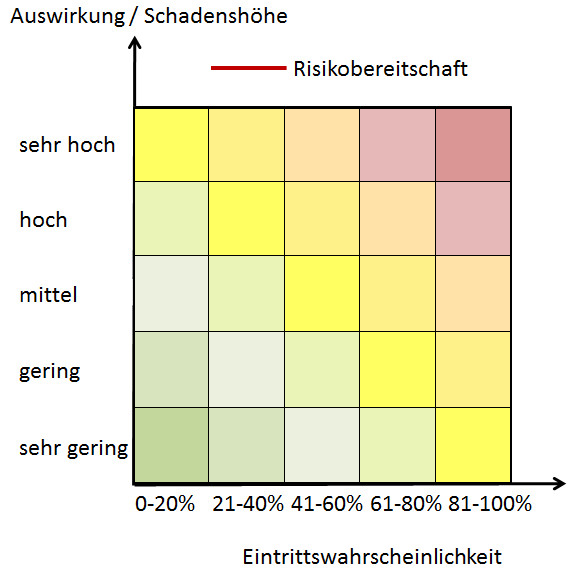
\includegraphics[width=0.75\textwidth]{src/risikomatrix.png}
	\caption{Risikomatrix}
	\label{fig:Matrixtable}
\end{figure}



\subsection{Projektüberwachung}\label{3.4-controlling}
{\em Wie wird der Projektstatus verfolgt? Wie stellt Ihr sicher, dass
  der Phasenleiter jederzeit über den Stand der Entwicklung informiert
  ist? Wie werden Probleme bzw. Verzögerungen frühzeitig erkannt und
  angegangen?}

Wir treffen uns mindst. einmal die Woche und geben den Status quo wider. Bei Anomalien wird sofort benachrichtigt, gewarnt und gehandelt, damit man eventuell Krisensitzungen abhalten kann. Notfalls wird eine Skype-Videokonferenz abgehalten, wenn es nicht anders geht.\\
Im Blockkurs werden wir uns an die Meilensteine (grob) richten. Alle 2h wird der derzeitige Stand (kurz) geschildert. Ebenso Vorschläge als auch Probleme bzw. Prognosen zu zukünftigen Problemen, da 12 Augen mehr erblicken können, als nur ein Einzelner.\\ 

\subsection{Mitarbeiter}
{\em Kompetenzen der und Anforderungen an die Mitarbeiter.}

Die Anzahl der Anforderungen ist - in diesem Fall - recht überschaubar, jedoch im Detail komplex.\\
Ein Minimum an Java-Kenntnissen reicht nur in der Theorie aus. Objektorientierung, Fehleranalyse und Kreation von effizienten Algorithmen, sollte man auch vorweisen können, da kein Kunde gerne 10min wartet, bis eine große Datenbank geladen hat und die Werte erst dann auf dem Bildschirm darstellt.\\
Natürlich ist es nicht der Standard. Es wird (verständlicherweise) immer Gruppenmitglieder geben, die eine Sache nicht vorweisen können.\\
Um dieser Lage Herr zu werden, ist eine optimale Aufgabenaufteilung erforderlich. Dazu später mehr [\ref{sec:arbeitspaket_zeitplan_budegt}]\\

Beobachtung und Analyse wären auch sehr empfehlenswert, wenn man später die Anforderungsspezifikation erstellen muss und in der Ist-/Soll-Phase, Personas-Phase, ... sich befindet. Da es keine richtigen Anforderungen sind und langsam am Thema vorbei geschrieben wird, wird dieser Aspekt offen in dem Raum gestellt.\\ 



%%%%%%%%%%%%%%%%%%%%%%%%%%%%%%%%%%%%%%%%%%%%%%%%%%%%%%%%%%%%%%%%%%%%%%%%

\section{Technische Prozesse}
\nurlangversion
\subsection{Methoden, Werkzeuge und Techniken}
\nurlangversion
\subsubsection{Entwicklungsplattform}

\subsubsection{Entwicklungsmethode}
{\em Ist der Einsatz spezieller Methoden vorgesehen?}

\subsubsection{Programmiersprache und Bibliotheken}

\subsection{Dokumentationsplan}
\nurlangversion

\subsubsection{Codingstyle}

\subsubsection{Kommentarsprache}

\subsubsection{JavaDoc}

\subsubsection{Begleitende Dokumentation}

\subsection{Unterstützende Projektfunktionen}
\nurlangversion
{\em Wie wird Euer Konfigurationsmanagement funktionieren? Wer ist verantwortlich? Benötigt Ihr dazu Ressourcen oder Zeit? Plant Ihr Datensicherung?}

{\em Gibt es Maßnahmen zur Qualitätssicherung? Wer ist zuständig?
  Wieviel Zeit ist dafür vorgesehen?}


%%%%%%%%%%%%%%%%%%%%%%%%%%%%%%%%%%%%%%%%%%%%%%%%%%%%%%%%%%%%%%%%%%%%%%%%

\section{Arbeitspakete, Zeitplan und Budget} 
\label{sec:arbeitspaket_zeitplan_budegt}

{\em Dieser Teil ist ein zweiter Schwerpunkt des Projektplans. Hier sollt Ihr die nächste Phase detailliert planen (siehe Arbeitspakete). Die weiteren Phasen sollen ebenfalls wenigstens grob geplant werden. Ein Gantt-Diagramm ist zwingend! 

Ihr sollt den Plan in der kommenden Phase auch tatsächlich benutzen -- und so
  Erfahrungen sammeln, was evtl. bei der Planung unberücksichtigt
  blieb. Bei der nächsten Zeitplanung (für die nächste Phase) bekommt
  Ihr dann evtl.\ eine noch bessere Planung hin.}

\subsection{Arbeitspakete}\label{aps}


{\em Besonderen Wert legen wir auf die Granularität der APs. Diese
  sollten von 1-2 Personen in max. einer Woche Zeitdauer (kalendarisch, nicht
  Aufwand) bearbeitbar sein. Die Beschreibungen sollten so genau sein,
  dass der Bearbeiter damit genau weiß, was zu tun ist.}
  

\begin{tabular}{|p{5.3cm}|p{9.7cm}|}\hline
	\textbf{Arbeitspaket Nr.:} 1.0 & \textbf{Bezeichnung:} Anforderungsspezifikation\\ \hline \hline
	\textbf{Beginn} & 01.06.14\\ \hline
	\textbf{Ende} & 06.07.14\\ \hline
	\textbf{Verantwortlicher} & \\ \hline
	\textbf{Ressourcen} & \begin{itemize}
		\item bla
		\item blaa
	\end{itemize}    \\ \hline
	\textbf{Abhängigkeit} &\\ \hline
	\textbf{Aufwand} & \\ \hline
	\textbf{Dauer} & \\ \hline
	\multicolumn{2}{|p{15cm}|}{\textbf{Beschreibung:}\newline   }\\ \hline
	\multicolumn{2}{|p{15cm}|}{\textbf{Mindestkriterien:}\newline }\\ \hline
\end{tabular}

\begin{verbatim} 
\end{verbatim}

\begin{tabular}{|p{5.3cm}|p{9.7cm}|}\hline
	\textbf{Arbeitspaket Nr.:} 1.0 & \textbf{Bezeichnung:} Gruppentreffen\\ \hline \hline
	\textbf{Beginn} & 01.06.14\\ \hline
	\textbf{Ende} &  01.07.14\\ \hline
	\textbf{Verantwortlicher} Alle \\ \hline
	\textbf{Ressourcen} & \begin{itemize}
		\item 
		\item blaa
	\end{itemize}    \\ \hline
	\textbf{Abhängigkeit} &\\ \hline
	\textbf{Aufwand} & 8h\\ \hline
	\textbf{Dauer} & ?\\ \hline
	\multicolumn{2}{|p{15cm}|}{\textbf{Beschreibung:}\newline  Um die Qualität der einzelnen Bearbeitungen sicherzustellen und eine Möglichkeit für Fragen und Besprechungen zu bieten, werden wir uns als Gruppe mindestens einmal in der Woche gemeinsam treffen. }\\ \hline
	\multicolumn{2}{|p{15cm}|}{\textbf{Mindestkriterien:}\newline Jeder Arbeitsvorgang kann bei Bedarf ausreichend für die weitere Bearbeitung besprochen werden. }\\ \hline
\end{tabular}

\begin{verbatim} 
\end{verbatim}

\begin{tabular}{|p{5.3cm}|p{9.7cm}|}\hline
	\textbf{Arbeitspaket Nr.:} 1.0 & \textbf{Bezeichnung:} GUI-Erstellung\\ \hline \hline
	\textbf{Beginn} & 02.06.14\\ \hline
	\textbf{Ende} & 16.06.14\\ \hline
	\textbf{Verantwortlicher} & Tobias Dellert\\ \hline
	\textbf{Ressourcen} & \begin{itemize}
		\item Alexander But
	\end{itemize}    \\ \hline
	\textbf{Abhängigkeit} &\\ \hline
	\textbf{Aufwand} & 16h\\ \hline
	\textbf{Dauer} & \\ \hline
	\multicolumn{2}{|p{15cm}|}{\textbf{Beschreibung:} Der hier erstellte Prototyp soll die Beschaffenheit der späteren Benutzeroberfläche darstellen. \newline   }\\ \hline
	\multicolumn{2}{|p{15cm}|}{\textbf{Mindestkriterien:} Der Kunde ist mit dem Prototypen einverstanden.\newline }\\ \hline
\end{tabular}

\begin{verbatim} 
\end{verbatim}

\begin{tabular}{|p{5.3cm}|p{9.7cm}|}\hline
	\textbf{Arbeitspaket Nr.:} 1.0 & \textbf{Bezeichnung:} Story-Board\\ \hline \hline
	\textbf{Beginn} & 02.06.14\\ \hline
	\textbf{Ende} & 02.06.14\\ \hline
	\textbf{Verantwortlicher} & Tobias Dellert\\ \hline
	\textbf{Ressourcen} & \begin{itemize}
		\item Tobias Dellert
	\end{itemize}    \\ \hline
	\textbf{Abhängigkeit} & -\\ \hline
	\textbf{Aufwand} & 1h\\ \hline
	\textbf{Dauer} & 1 Tag\\ \hline
	\multicolumn{2}{|p{15cm}|}{\textbf{Beschreibung:}\newline  Das Story-Board beschreibt die erforderlichen Darstellungen, um die möglichen Vorgänge abzudecken }\\ \hline
	\multicolumn{2}{|p{15cm}|}{\textbf{Mindestkriterien:}\newline Alle mögliche Vorgänge sind abgedeckt. }\\ \hline
\end{tabular}

\begin{verbatim} 
\end{verbatim}

\begin{tabular}{|p{5.3cm}|p{9.7cm}|}\hline
	\textbf{Arbeitspaket Nr.:} 1.0 & \textbf{Bezeichnung:} Design\\ \hline \hline
	\textbf{Beginn} & 03.02.14\\ \hline
	\textbf{Ende} & 03.02.14\\ \hline
	\textbf{Verantwortlicher} & Alexander But\\ \hline
	\textbf{Ressourcen} & \begin{itemize}
		\item Alexander But
	\end{itemize}    \\ \hline
	\textbf{Abhängigkeit} & -\\ \hline
	\textbf{Aufwand} & 4h\\ \hline
	\textbf{Dauer} & 1 Tag\\ \hline
	\multicolumn{2}{|p{15cm}|}{\textbf{Beschreibung:}Hier werden die einzelnen Bestandteile des Prototypen gestaltet.\newline   }\\ \hline
	\multicolumn{2}{|p{15cm}|}{\textbf{Mindestkriterien:} Das Design soll den Wünschen des Kunden bestmöglich entsprechen\newline }\\ \hline
	
\end{tabular}
\begin{verbatim} 

\end{verbatim}
\begin{tabular}{|p{5.3cm}|p{9.7cm}|}\hline
	\textbf{Arbeitspaket Nr.:} 1.0 & \textbf{Bezeichnung:} Entwicklungsphase I \\ \hline \hline
	\textbf{Beginn} & 04.01.14\\ \hline
	\textbf{Ende} & 06.01.15\\ \hline
	\textbf{Verantwortlicher} & Tobias Dellert \\ \hline
	\textbf{Ressourcen} & \begin{itemize}
		\item Tobias Dellert
		\item Alexander But
	\end{itemize}    \\ \hline
	\textbf{Abhängigkeit} & Story-Board, Design\\ \hline
	\textbf{Aufwand} & 16h\\ \hline
	\textbf{Dauer} & 3 Tage\\ \hline
	\multicolumn{2}{|p{15cm}|}{\textbf{Beschreibung:}\newline Das Konzept von Stroy-Board und Design wird umgesetzt. Die Ergebnisse der ersten Entwicklungsphase werden dem Kunden vorgestellt.  }\\ \hline
	\multicolumn{2}{|p{15cm}|}{\textbf{Mindestkriterien:}\newline Die Entwicklungsphase ist ein Ergebnis aus dem Story-Board und dem Design, welche auf dem Verständnis der Wünsche des Kunden basieren.}\\ \hline
	
\end{tabular}
\begin{verbatim} 

\end{verbatim}
\begin{tabular}{|p{5.3cm}|p{9.7cm}|}\hline
	\textbf{Arbeitspaket Nr.:} 1.0 & \textbf{Bezeichnung:} GUI-Prototyp-Vorstellung\\ \hline \hline
	\textbf{Beginn} & 11.06.14\\ \hline
	\textbf{Ende} &11.06.14\\ \hline
	\textbf{Verantwortlicher} & Tobias Dellert\\ \hline
	\textbf{Ressourcen} & \begin{itemize}
		\item Tobias Dellert
		\item Alexander But
	\end{itemize}    \\ \hline
	\textbf{Abhängigkeit} & Entwicklungsphase I\\ \hline
	\textbf{Aufwand} & 6h\\ \hline
	\textbf{Dauer} & 1 Tag\\ \hline
	\multicolumn{2}{|p{15cm}|}{\textbf{Beschreibung:}\newline  Das Ergebnis der ersten Entwicklungsphase wird dem Kunden vorgestellt. Es wird bestmöglich versucht die Meinung des Kunden dazu und eventuelle Verbesserungswünsche zu verstehen. }\\ \hline
	\multicolumn{2}{|p{15cm}|}{\textbf{Mindestkriterien:}\newline Die Meinung des Kunden wurde erfasst und das weitere Vorgehen beim GUI-Prototypen ist klar.}\\ \hline
	
\end{tabular}
\begin{verbatim} 

\end{verbatim}
\begin{tabular}{|p{5.3cm}|p{9.7cm}|}\hline
	\textbf{Arbeitspaket Nr.:} 1.0 & \textbf{Bezeichnung:} Entwicklungsphase II\\ \hline \hline
	\textbf{Beginn} & 12.06.14\\ \hline
	\textbf{Ende} & 16.06.14\\ \hline
	\textbf{Verantwortlicher} & Alexander But\\ \hline
	\textbf{Ressourcen} & \begin{itemize}
		\item Tobias Dellert
	\end{itemize}    \\ \hline
	\textbf{Abhängigkeit} & GUI-Prototyp-Vorstellung\\ \hline
	\textbf{Aufwand} & 8h\\ \hline
	\textbf{Dauer} & 5 tage\\ \hline
	\multicolumn{2}{|p{15cm}|}{\textbf{Beschreibung:}\newline  Der Prototyp wird gegebenenfalls angepasst. }\\ \hline
	\multicolumn{2}{|p{15cm}|}{\textbf{Mindestkriterien:}\newline Die Erkenntnisse aus der Prototyp-Vorstellung werden umgesetzt.}\\ \hline
\end{tabular}

\begin{verbatim} 
\end{verbatim}

\begin{tabular}{|p{5.3cm}|p{9.7cm}|}\hline
	\textbf{Arbeitspaket Nr.:} 1.0 & \textbf{Bezeichnung:} Dokument der Anforderungsspezifikation\\ \hline \hline
	\textbf{Beginn} & 04.06.14\\ \hline
	\textbf{Ende} & 04.07.14\\ \hline
	\textbf{Verantwortlicher} & Alle\\ \hline
		\textbf{Ressourcen} & \begin{itemize}
			\item Alle
		\end{itemize}    \\ \hline
		\textbf{Abhängigkeit} &\\ \hline
		\textbf{Aufwand} & 79h\\ \hline
		\textbf{Dauer} & 30 tage\\ \hline
		\multicolumn{2}{|p{15cm}|}{\textbf{Beschreibung:} Im Dokument werden die Anforderungen an das System dargestellt, was grundlegend für die weitere Entwicklung in unserem Projekt ist. Es wird eine Gespräch bezüglich der Wünsche abgehalten, ähnliche Systeme werden untersucht und verglichen, und die gewonnenen Erkenntnisse werden anwendungsbezogen dargestellt.\newline   }\\ \hline
		\multicolumn{2}{|p{15cm}|}{\textbf{Mindestkriterien:}\newline Das Dokument stellt die Wünsche des Kunden ausreichend dar, um aufgrund dessen eine gelungene Architektur zu entwerfen.}\\ \hline
	\end{tabular}
	
	\begin{verbatim} 
	\end{verbatim}
	
	\begin{tabular}{|p{5.3cm}|p{9.7cm}|}\hline
		\textbf{Arbeitspaket Nr.:} 1.0 & \textbf{Bezeichnung:} Allgemeine Beschreibung\\  \hline \hline
		\textbf{Beginn} & 03.06.14\\ \hline
		\textbf{Ende} & 09.06.14\\ \hline
		\textbf{Verantwortlicher} & Karsten Betjemann\\ \hline
		\textbf{Ressourcen} & \begin{itemize}
			\item Tim Ellhoff
			\item Tobias Dellert
			\item Karsten Betjemann
			\item Alexander But
		\end{itemize}    \\ \hline
		\textbf{Abhängigkeit} & \\ \hline
		\textbf{Aufwand} & 23h \\ \hline
		\textbf{Dauer} & 6 Tage\\ \hline
		\multicolumn{2}{|p{15cm}|}{\textbf{Beschreibung:}\newline Um den bisherigen Zustand bezüglich bestehender Anforderungen oder Wünsche des Kunden zu erfassen, wird sowohl ein Gespräch geführt, als auch zuvor ein Vergleich mit ähnlichen Systemen durchgeführt.   }\\ \hline
		\multicolumn{2}{|p{15cm}|}{\textbf{Mindestkriterien:}\newline Die Anforderungen und Wünsche des Kunden werden erfasst.}\\ \hline
	\end{tabular}
	
	\begin{verbatim} 
	\end{verbatim}
	
	\begin{tabular}{|p{5.3cm}|p{9.7cm}|}\hline
		\textbf{Arbeitspaket Nr.:} 1.0 & \textbf{Bezeichnung:} Ausführung der Ist-Analyse\\  \hline \hline
		\textbf{Beginn} & 03.06.14\\ \hline
		\textbf{Ende} & 09.06.14\\ \hline
		\textbf{Verantwortlicher} & Karsten Betjemann\\ \hline
		\textbf{Ressourcen} & \begin{itemize}
			\item Tim Ellhoff
			\item Tobias Dellert
			\item Karsten Betjemann
			\item Alexander But
		\end{itemize}    \\ \hline
		\textbf{Abhängigkeit} & \\ \hline
		\textbf{Aufwand} & 13h\\ \hline
		\textbf{Dauer} & 6 Tage\\ \hline
		\multicolumn{2}{|p{15cm}|}{\textbf{Beschreibung:}\newline Um den bisherigen Zustand bezüglich bestehender Anforderungen oder Wünsche des Kunden zu erfassen, wird sowohl ein Gespräch geführt, als auch zuvor ein Vergleich mit ähnlichen Systemen durchgeführt.   }\\ \hline
		\multicolumn{2}{|p{15cm}|}{\textbf{Mindestkriterien:}\newline Die Anforderungen und Wünsche des Kunden werden erfasst.}\\ \hline
	\end{tabular}
	
	\begin{verbatim} 
	\end{verbatim}
	
	\begin{tabular}{|p{5.3cm}|p{9.7cm}|}\hline
		\textbf{Arbeitspaket Nr.:} 1.0 & \textbf{Bezeichnung:} Analyse ähnlicher Systeme\\ \hline \hline
		\textbf{Beginn} & 03.06.14\\ \hline
		\textbf{Ende} & 04306.14\\ \hline
		\textbf{Verantwortlicher} & Karsten Betjemann\\ \hline
		\textbf{Ressourcen} & \begin{itemize}
			\item Karsten Betjemann
		\end{itemize}    \\ \hline
		\textbf{Abhängigkeit} &\\ \hline
		\textbf{Aufwand} & 3h\\ \hline
		\textbf{Dauer} & 1 Tag\\ \hline
		\multicolumn{2}{|p{15cm}|}{\textbf{Beschreibung:}\newline Es werden die Funktionen und daraus folgenden Vor- und Nachteile abgewogen, um später diese mit den Anforderungen des Kunden zu vergleichen.}\\ \hline
		\multicolumn{2}{|p{15cm}|}{\textbf{Mindestkriterien:}\newline Es wird mindestens ein ähnliches System analysiert}\\ \hline   
	\end{tabular}
	
	\begin{verbatim} 
	\end{verbatim}
	
	\begin{tabular}{|p{5.3cm}|p{9.7cm}|}\hline
		\textbf{Arbeitspaket Nr.:} 1.0 & \textbf{Bezeichnung:} Vorbereitung auf das Kundengespräch\\ \hline \hline
		\textbf{Beginn} & 04.06.14\\ \hline
		\textbf{Ende} & 04.06.14\\ \hline
		\textbf{Verantwortlicher} & Karsten Betjemann\\ \hline
		\textbf{Ressourcen} & \begin{itemize}
			\item Tobias Dellert
			\item Alexander But
			\item Karsten Betjemann
		\end{itemize}    \\ \hline
		\textbf{Abhängigkeit} &\\ \hline
		\textbf{Aufwand} & 3h\\ \hline
		\textbf{Dauer} & 1 Tag\\ \hline
		\multicolumn{2}{|p{15cm}|}{\textbf{Beschreibung:}\newline Es werden eventuell offene Fragen zur den Anforderungen und dessen Durchführungen notiert. Unter anderem auch  basierend auf den Erkenntnissen der vorherigen Analyse ähnlicher Systeme. }\\ \hline
		\multicolumn{2}{|p{15cm}|}{\textbf{Mindestkriterien:}\newline Der erhaltene Fragenkatalog enthält die wichtigsten zu besprechende Punkt. }\\ \hline
	\end{tabular}
	
	\begin{verbatim} 
	\end{verbatim}
	
	\begin{tabular}{|p{5.3cm}|p{9.7cm}|}\hline
		\textbf{Arbeitspaket Nr.:}  & \textbf{Bezeichnung:} Kundengespräch\\ \hline \hline
		\textbf{Beginn} & 05.06.14\\ \hline
		\textbf{Ende} & 05.06.14\\ \hline
		\textbf{Verantwortlicher} & Tobias Dellert\\ \hline
		\textbf{Ressourcen} & \begin{itemize}
			\item Tobias Dellert
			\item Alexander But
		\end{itemize}    \\ \hline
		\textbf{Abhängigkeit} &\\ \hline
		\textbf{Aufwand} & 6h\\ \hline
		\textbf{Dauer} & 1 Tag\\ \hline
		\multicolumn{2}{|p{15cm}|}{\textbf{Beschreibung:}\newline Anhand des Fragenkataloges werden diese und vermutlich noch aufkommende Fragen dem Kunden gestellt. }\\ \hline
		\multicolumn{2}{|p{15cm}|}{\textbf{Mindestkriterien:}\newline Am Ende sollen alle Fragen geklärt worden sein. }\\ \hline
	\end{tabular}
	
	\begin{verbatim} 
	\end{verbatim}
	
	\begin{tabular}{|p{5.3cm}|p{9.7cm}|}\hline
		\textbf{Arbeitspaket Nr.:}  & \textbf{Bezeichnung:} Auswertung des Kundengesprächs\\ \hline \hline
		\textbf{Beginn} & 05.06.14\\ \hline
		\textbf{Ende} & 05.06.14\\ \hline
		\textbf{Verantwortlicher} & Alexander But\\ \hline
		\textbf{Ressourcen} & \begin{itemize}
			\item Alexander But
			\item Tobias Dellert
		\end{itemize}    \\ \hline
		\textbf{Abhängigkeit} & Kundengespräch\\ \hline
		\textbf{Aufwand} & 1h\\ \hline
		\textbf{Dauer} & 1 Tag\\ \hline
		\multicolumn{2}{|p{15cm}|}{\textbf{Beschreibung:}\newline Die Beantwortungen der Fragen werden Zusammengesetzt und mit den bestehenden Mindestanforderungen in Verbindung gebracht. }\\ \hline
		\multicolumn{2}{|p{15cm}|}{\textbf{Mindestkriterien:}\newline Es soll ein umfassendes Bild der Anforderungen erlangt worden sein. }\\ \hline
	\end{tabular}
	
	\begin{verbatim} 
	\end{verbatim}
	
	\begin{tabular}{|p{5.3cm}|p{9.7cm}|}\hline
		\textbf{Arbeitspaket Nr.:}  & \textbf{Bezeichnung:} Ausführung der Soll-Analyse\\ \hline \hline
		\textbf{Beginn} & 09.06.14\\ \hline
		\textbf{Ende} & 16.06.14\\ \hline
		\textbf{Verantwortlicher} & Tim Ellhoff\\ \hline
		\textbf{Ressourcen} & \begin{itemize}
			\item Tim Ellhoff
			\item Karsten Betjemann
		\end{itemize}    \\ \hline
		\textbf{Abhängigkeit} & Ausführung der Ist-Analyse\\ \hline
		\textbf{Aufwand} & 10h\\ \hline
		\textbf{Dauer} & 8 Tage\\ \hline
		\multicolumn{2}{|p{15cm}|}{\textbf{Beschreibung:}\newline Die Erkenntnisse aus dem Kundegespräch ermöglichen eine gute und zutreffende Interpretation der gestellten Anforderungen. Diese werden hier in Form von einfachen Anwendungsfällen beschrieben werden. Zudem werden die Rahmenbedingungen zur Ausführung festgelegt. }\\ \hline
		\multicolumn{2}{|p{15cm}|}{\textbf{Mindestkriterien:}\newline Die Wünsche des Kunden sind in dem beschriebenen Soll-Zustand zutreffend dargestellt. }\\ \hline
	\end{tabular}
	
	\begin{verbatim} 
	\end{verbatim}
	
	\begin{tabular}{|p{5.3cm}|p{9.7cm}|}\hline
		\textbf{Arbeitspaket Nr.:}  & \textbf{Bezeichnung:} Produktperspektiven\\ \hline \hline
		\textbf{Beginn} & 09.0.14\\ \hline
		\textbf{Ende} & 11.06.14\\ \hline
		\textbf{Verantwortlicher} & Karsten Betjemann\\ \hline
		\textbf{Ressourcen} & \begin{itemize}
			\item Karsten Betjemann
			\item Tim Ellhoff
		\end{itemize}    \\ \hline
		\textbf{Abhängigkeit} & Kundengespräch\\ \hline
		\textbf{Aufwand} & 3h\\ \hline
		\textbf{Dauer} & 2 Tage\\ \hline
		\multicolumn{2}{|p{15cm}|}{\textbf{Beschreibung:}\newline Hier werden die grundlegenden Rahmenbedingungen zusammengestellt um für den weiteren Projektverlauf realistische Planungen durchführen zu können. }\\ \hline
		\multicolumn{2}{|p{15cm}|}{\textbf{Mindestkriterien:}\newline Alle wichtigen und sytsembetreffende Bereiche wurden beachtet. }\\ \hline
	\end{tabular}
	
	\begin{verbatim} 
	\end{verbatim}
	
	
	\begin{tabular}{|p{5.3cm}|p{9.7cm}|}\hline
		\textbf{Arbeitspaket Nr.:}  & \textbf{Bezeichnung:} Einschränkungen\\ \hline \hline
		\textbf{Beginn} & 12.06.14\\ \hline
		\textbf{Ende} & 12.06.14\\ \hline
		\textbf{Verantwortlicher} & Karsten Betjemann\\ \hline
		\textbf{Ressourcen} & \begin{itemize}
			\item Karsten Betjemann
		\end{itemize}    \\ \hline
		\textbf{Abhängigkeit} &\\ \hline
		\textbf{Aufwand} & 1h\\ \hline
		\textbf{Dauer} & 1 Tag\\ \hline
		\multicolumn{2}{|p{15cm}|}{\textbf{Beschreibung:}\newline Die technischen und rechtlichen Einschränkungen während der Durchführung des Projektes und Ausführung der 
			fertigen Software werden erfasst. }\\ \hline
		\multicolumn{2}{|p{15cm}|}{\textbf{Mindestkriterien:}\newline Die Einschränkungen wurden soweit erfasst, dass das Projekt technisch und rechtlich durchführbar ist. }\\ \hline
	\end{tabular}
	
	\begin{verbatim} 
	\end{verbatim}
	
	\begin{tabular}{|p{5.3cm}|p{9.7cm}|}\hline
		\textbf{Arbeitspaket Nr.:}  & \textbf{Bezeichnung:} Allgemeine Anwendungsfälle\\ \hline \hline
		\textbf{Beginn} & 12.06.14\\ \hline
		\textbf{Ende} & 16.06.14\\ \hline
		\textbf{Verantwortlicher} & Tim Ellhoff\\ \hline
		\textbf{Ressourcen} & \begin{itemize}
			\item Tim Ellhoff
			\item Karsten Betjemann
		\end{itemize}    \\ \hline
		\textbf{Abhängigkeit} &\\ \hline
		\textbf{Aufwand} & 4h \\ \hline
		\textbf{Dauer} & 5 Tage\\ \hline
		\multicolumn{2}{|p{15cm}|}{\textbf{Beschreibung:} siehe Unterpunkte\newline  }\\ \hline
		\multicolumn{2}{|p{15cm}|}{\textbf{Mindestkriterien:}\newline Die Anwendungsfälle decken die möglichen Vorgänge im gewünschten System ab. }\\ \hline
	\end{tabular}
	
	\begin{verbatim} 
	\end{verbatim}
	
	\begin{tabular}{|p{5.3cm}|p{9.7cm}|}\hline
		\textbf{Arbeitspaket Nr.:}  & \textbf{Bezeichnung:} Liste der Anwendungsfälle\\ \hline \hline
		\textbf{Beginn} & 12.0.14\\ \hline
		\textbf{Ende} & 13.06.14\\ \hline
		\textbf{Verantwortlicher} & Tim Ellhoff\\ \hline
		\textbf{Ressourcen} & \begin{itemize}
			\item Tim Ellhoff 
		\end{itemize}    \\ \hline
		\textbf{Abhängigkeit} &\\ \hline
		\textbf{Aufwand} & 2h\\ \hline
		\textbf{Dauer} & 2 Tage\\ \hline
		\multicolumn{2}{|p{15cm}|}{\textbf{Beschreibung:}\newline Die allgemein gehaltenen Anwendungsfälle beschreiben den Vorgang in der späteren Software.}\\ \hline
		\multicolumn{2}{|p{15cm}|}{\textbf{Mindestkriterien:}\newline siehe Oberpunkt. }\\ \hline
	\end{tabular}
	
	\begin{verbatim} 
	\end{verbatim}
	
	\begin{tabular}{|p{5.3cm}|p{9.7cm}|}\hline
		\textbf{Arbeitspaket Nr.:}  & \textbf{Bezeichnung:} Erstellung der Charakteristika\\ \hline \hline
		\textbf{Beginn} & 13.06.14\\ \hline
		\textbf{Ende} & 16.06.14\\ \hline
		\textbf{Verantwortlicher} & Tim Ellhoff\\ \hline
		\textbf{Ressourcen} & \begin{itemize}
			\item Tim Ellhoff
		\end{itemize}    \\ \hline
		\textbf{Abhängigkeit} &\\ \hline
		\textbf{Aufwand} & 2h\\ \hline
		\textbf{Dauer} & 2 Tage\\ \hline
		\multicolumn{2}{|p{15cm}|}{\textbf{Beschreibung:}\newline Es werden typisch denkbare Personen in der Rolle als Nutzer der Software erstellt. Die Personen sollen helfen sich in die Lage zukünftiger Nutzer hineinzuversetzen, da jede dieser Personen unterschiedliche Prioritäten besitzt, die mit der Software aber verfolgbar sein sollen. }\\ \hline
		\multicolumn{2}{|p{15cm}|}{\textbf{Mindestkriterien:}\newline Die Software wird typischen Nutzern gerecht. }\\ \hline
	\end{tabular}
	
	\begin{verbatim} 
	\end{verbatim}
	
	\begin{tabular}{|p{5.3cm}|p{9.7cm}|}\hline
		\textbf{Arbeitspaket Nr.:}  & \textbf{Bezeichnung:} Ausblick in die Zukunft\\ \hline \hline
		\textbf{Beginn} & 17.0.14\\ \hline
		\textbf{Ende} & 19.06.14\\ \hline
		\textbf{Verantwortlicher} & \\ \hline
		\textbf{Ressourcen} & \begin{itemize}
			\item Tim Ellhoff 
		\end{itemize}    \\ \hline
		\textbf{Abhängigkeit} &\\ \hline
		\textbf{Aufwand} & 2h\\ \hline
		\textbf{Dauer} & 3 Tage\\ \hline
		\multicolumn{2}{|p{15cm}|}{\textbf{Beschreibung:}\newline Hier werden zu erwartende Änderungen softwarebeeinflussender Faktoren wie Datenschutzrecht und technische Weiterentwicklungen und deren Einfluss auf unser Projekt und System betrachtet. }\\ \hline
		\multicolumn{2}{|p{15cm}|}{\textbf{Mindestkriterien:}\newline Der Ausblick war umfassen genug und gab Beiträge zu eventueller Anpassung der Durchführung unseres Projekts in Sachen Wartbar- und Erweiterbarkeit. }\\ \hline
	\end{tabular}
	
	\begin{verbatim} 
	\end{verbatim}
	
	\begin{tabular}{|p{5.3cm}|p{9.7cm}|}\hline
		\textbf{Arbeitspaket Nr.:}  & \textbf{Bezeichnung:} Detaillierte Beschreibung\\ \hline \hline
		\textbf{Beginn} & 23.06.14\\ \hline
		\textbf{Ende} & 02.07.14\\ \hline
		\textbf{Verantwortlicher} & Alle\\ \hline
		\textbf{Ressourcen} & \begin{itemize}
			\item Alle
		\end{itemize}    \\ \hline
		\textbf{Abhängigkeit} & Allgemeine Beschreibung\\ \hline
		\textbf{Aufwand} & 56h\\ \hline
		\textbf{Dauer} & 10 Tage\\ \hline
		\multicolumn{2}{|p{15cm}|}{\textbf{Beschreibung:} Hier werden unter Anderem die Anwendungsfälle spezifiziert und mit den entspechenden GUI-Oberflächen versehen. 
			Detaillierungen unterstützen den späteren Übergang der Konzepte der Anforderungsspezifikation in die technische Sicht der Architektur.\newline  }\\ \hline
		\multicolumn{2}{|p{15cm}|}{\textbf{Mindestkriterien:}\newline  }\\ \hline
	\end{tabular}
	
	\begin{verbatim} 
	\end{verbatim}
	
	\begin{tabular}{|p{5.3cm}|p{9.7cm}|}\hline
		\textbf{Arbeitspaket Nr.:}  & \textbf{Bezeichnung:} Datenmodell\\ \hline \hline
		\textbf{Beginn} & 23.06.14\\ \hline
		\textbf{Ende} & 26.06.14\\ \hline
		\textbf{Verantwortlicher} & Tobias Dellert\\ \hline
		\textbf{Ressourcen} & \begin{itemize}
			\item Tobias Dellert
		\end{itemize}    \\ \hline
		\textbf{Abhängigkeit} &\\ \hline
		\textbf{Aufwand} 6h & \\ \hline
		\textbf{Dauer} & 3 Tage\\ \hline
		\multicolumn{2}{|p{15cm}|}{\textbf{Beschreibung:}\newline Das Datenmodell beschreibt einen Ausschnitt der realen Welt in Form vom Austausch von Informationen verschiedener Klassen. Dieses Modell wird als UML-KLassendiagramm erstellt und bezieht sich auf ein fachlogisches Konzept, ohne Implementierungsdetails. }\\ \hline
		\multicolumn{2}{|p{15cm}|}{\textbf{Mindestkriterien:}\newline Das Datenmodell beschreibt den Informationsfluss treffend und einfach. }\\ \hline
	\end{tabular}
	
	\begin{verbatim} 
	\end{verbatim}
	
	\begin{tabular}{|p{5.3cm}|p{9.7cm}|}\hline
		\textbf{Arbeitspaket Nr.:}  & \textbf{Bezeichnung:} Detaillierte Anwendungsfälle\\ \hline \hline
		\textbf{Beginn} & 24.06.14\\ \hline
		\textbf{Ende} & 30.06.14\\ \hline
		\textbf{Verantwortlicher} & Alle\\ \hline
		\textbf{Ressourcen} & \begin{itemize}
			\item Alle
		\end{itemize}    \\ \hline
		\textbf{Abhängigkeit} & Allgemeine Anwendungsfälle\\ \hline
		\textbf{Aufwand} & 40h\\ \hline
		\textbf{Dauer} & 7 Tage\\ \hline
		\multicolumn{2}{|p{15cm}|}{\textbf{Beschreibung:}\newline Hier werden die Anwendungsfälle detailliert und mit Screenshots der GUI-Oberfläche versehen. }\\ \hline
		\multicolumn{2}{|p{15cm}|}{\textbf{Mindestkriterien:}\newline Die Anwendungsfälle stellen alle möglichen Vorgänge des späteren Systems dar. }\\ \hline
	\end{tabular}
	
	\begin{verbatim} 
	\end{verbatim}
	
	\begin{tabular}{|p{5.3cm}|p{9.7cm}|}\hline
		\textbf{Arbeitspaket Nr.:}  & \textbf{Bezeichnung:} Aktionen\\ \hline \hline
		\textbf{Beginn} & 01.07.14\\ \hline
		\textbf{Ende} & 02.06.14\\ \hline
		\textbf{Verantwortlicher} & Alexander But\\ \hline
		\textbf{Ressourcen} & \begin{itemize}
			\item Alexander But
		\end{itemize}    \\ \hline
		\textbf{Abhängigkeit} & Detaillierte Anwendungsfälle\\ \hline
		\textbf{Aufwand} & 6h\\ \hline
		\textbf{Dauer} & 2 Tage\\ \hline
		\multicolumn{2}{|p{15cm}|}{\textbf{Beschreibung:}\newline Hier werden die detaillierteren Anwendungsfälle implemetierungsspezifisch dargestellt. Ihnen werden also zukünftige Methodennamen und Parameter zugeteilt, welche die entsprechende Methode für die Ausführung benötigen wird.  }\\ \hline
		\multicolumn{2}{|p{15cm}|}{\textbf{Mindestkriterien:}\newline  Allen Anwendungsfällen wurden Methoden und entsprechende Parameter zugeordnet. }\\ \hline
	\end{tabular}
	
	\begin{verbatim} 
	\end{verbatim}
	
	\begin{tabular}{|p{5.3cm}|p{9.7cm}|}\hline
		\textbf{Arbeitspaket Nr.:}  & \textbf{Bezeichnung:} Systemattribute\\ \hline \hline
		\textbf{Beginn} & 02.07.14\\ \hline
		\textbf{Ende} & 02.06.14\\ \hline
		\textbf{Verantwortlicher} & Tobias Dellert\\ \hline
		\textbf{Ressourcen} & \begin{itemize}
			\item Tobias Dellert 
		\end{itemize}    \\ \hline
		\textbf{Abhängigkeit} &\\ \hline
		\textbf{Aufwand} & 2h\\ \hline
		\textbf{Dauer} & 1 Tag\\ \hline
		\multicolumn{2}{|p{15cm}|}{\textbf{Beschreibung:}\newline Betrachtung der für die Implementierung benötigten Attribute. }\\ \hline
		\multicolumn{2}{|p{15cm}|}{\textbf{Mindestkriterien:}\newline Die Attribute decken die Anforderungen ab. }\\ \hline
	\end{tabular}
	
	\begin{verbatim} 
	\end{verbatim}
	
	\begin{tabular}{|p{5.3cm}|p{9.7cm}|}\hline
		\textbf{Arbeitspaket Nr.:}  & \textbf{Bezeichnung:} Schreiben des Angebotes\\ \hline \hline
		\textbf{Beginn} & 03.07.14\\ \hline
		\textbf{Ende} & 03.07.14\\ \hline
		\textbf{Verantwortlicher} & Tim Ellhoff\\ \hline
		\textbf{Ressourcen} & \begin{itemize}
			\item Tim Ellhoff
		\end{itemize}    \\ \hline
		\textbf{Abhängigkeit} & Fertigstellung des Dokuments\\ \hline
		\textbf{Aufwand} & 2h\\ \hline
		\textbf{Dauer} & 1 Tag\\ \hline
		\multicolumn{2}{|p{15cm}|}{\textbf{Beschreibung:}\newline Hier wird dem Kunden schriftlich ein Angebot unterbreitet, welche Kosten der Erwirb der gewünschten Software zuzuordnen ist. }\\ \hline
		\multicolumn{2}{|p{15cm}|}{\textbf{Mindestkriterien:}\newline Die Kostenberechnung wird im Dokument kurz erläutert und Formalitäten wurden beachtet. }\\ \hline
	\end{tabular}
	
	\begin{verbatim} 
	\end{verbatim}
	
	\textbf{Architekturbeschreibung und Implementierung:}\\
	Die anschließenden Pakete der Architektur und Implementierung sind hier lediglich grob unterteilt.
	
	\begin{tabular}{|p{5.3cm}|p{9.7cm}|}\hline
		\textbf{Arbeitspaket Nr.:}  & \textbf{Bezeichnung:} Erstellung der Architektur\\ \hline \hline
		\textbf{Beginn} & 07.07.14\\ \hline
		\textbf{Ende} & 25.07.14\\ \hline
		\textbf{Verantwortlicher} & Alle\\ \hline
		\textbf{Ressourcen} & \begin{itemize}
			\item Alle
		\end{itemize}    \\ \hline
		\textbf{Abhängigkeit} & Anforderungsspez.\\ \hline
		\textbf{Aufwand} & 120h\\ \hline
		\textbf{Dauer} & 19 Tage\\ \hline
		\multicolumn{2}{|p{15cm}|}{\textbf{Beschreibung:}\newline Die Konzepte der Anforderungsspez. werden in verschiedene technisch orientiertere Sichten unterteilt, die als Programmieranleitung dienen und insgesamt eine komplette Systemstruktur bildet.}\\ \hline
		\multicolumn{2}{|p{15cm}|}{\textbf{Mindestkriterien:}\newline Die Architektur ist wegweisend für die Implementierung. }\\ \hline
	\end{tabular}
	
	\begin{verbatim} 
	\end{verbatim}
	
	\begin{tabular}{|p{5.3cm}|p{9.7cm}|}\hline
		\textbf{Arbeitspaket Nr.:}  & \textbf{Bezeichnung:}Blackbox-Tests \\ \hline \hline
		\textbf{Beginn} & 23.07.14\\ \hline
		\textbf{Ende} & 24.07.14\\ \hline
		\textbf{Verantwortlicher} & Alle\\ \hline
		\textbf{Ressourcen} & \begin{itemize}
			\item Alle
		\end{itemize}    \\ \hline
		\textbf{Abhängigkeit} & Fertigstellung der Architektur\\ \hline
		\textbf{Aufwand} & 20h\\ \hline
		\textbf{Dauer} & \\ \hline
		\multicolumn{2}{|p{15cm}|}{\textbf{Beschreibung:}\newline Dieser Test achtet lediglich  auf die Korrektheit der Ergebnisse der Kommunikation zwischen den einzelnen Modulen. }\\ \hline
		\multicolumn{2}{|p{15cm}|}{\textbf{Mindestkriterien:}\newline Alle Schnittstellen wurden überprüft. }\\ \hline
	\end{tabular}
	
	\begin{verbatim} 
	\end{verbatim}
	
	\begin{tabular}{|p{5.3cm}|p{9.7cm}|}\hline
		\textbf{Arbeitspaket Nr.:}  & \textbf{Bezeichnung:} Implementierung\\ \hline \hline
		\textbf{Beginn} & 04.08.14\\ \hline
		\textbf{Ende} & 08.08.14\\ \hline
		\textbf{Verantwortlicher} & Alle\\ \hline
		\textbf{Ressourcen} & \begin{itemize}
			\item Alle
		\end{itemize}    \\ \hline
		\textbf{Abhängigkeit} & Architekturbeschreibung\\ \hline
		\textbf{Aufwand} & 100h\\ \hline
		\textbf{Dauer} & 5 Tage\\ \hline
		\multicolumn{2}{|p{15cm}|}{\textbf{Beschreibung:}\newline Implementierung der erstellten Programmstrukturen. }\\ \hline
		\multicolumn{2}{|p{15cm}|}{\textbf{Mindestkriterien:}\newline Die Mindestanforderungen sind im System realisiert. }\\ \hline
	\end{tabular}
	
	\begin{verbatim} 
	\end{verbatim}
	
	\subsection{Zeitplan und Abhängigkeiten}
	
	{\em Die Abhängigkeiten zwischen Arbeitspaketen oder Meilensteinen müssen genannt werden, sowie im
		Gantt-Diagramm eingezeichnet werden. Der kritische Pfad soll
		angegeben und/oder eingezeichnet werden!}
	
	\subsection{Ressourcenanforderung}
	
	{\em Jedem Arbeitspaket muss mind.\ ein Bearbeiter zugeordnet
		werden. Die Zuordnung der ganzen Gruppe sollte nur in Ausnahmefällen
		erfolgen -- und dann vermutlich begründet werden!}
	
	
	%%%%%%%%%%%%%%%%%%%%%%%%%%%%%%%%%%%%%%%%%%%%%%%%%%%%%%%%%%%%%%%%%%%%%%%%
\section{Sonstige Elemente}
\nurlangversion
\subsection{Pläne für die Konvertierung von Daten}
\nurlangversion

\subsection{Managementpläne für Unterauftragsnehmer}
\nurlangversion
{\em Wenn Fremdbibliotheken benutzt werden\dots}

\subsection{Ausbildungspläne}
\nurlangversion
{\em Hierunter fallen z.B. auch interne Schulungen, die Ihr
  durchführen wollt.}

\subsection{Raumpläne}
\nurlangversion
\dots

\subsection{Installationspläne}
\nurlangversion
\dots

\subsection{Pläne für die Übergabe des Systems}
\nurlangversion
\dots

\subsection{Beschaffungspläne für Hardware}
\nurlangversion
\dots


\end{document}
